\documentclass{article}
\usepackage[margin=.75in]{geometry}
\usepackage{graphicx, dblfloatfix}
\usepackage{amsmath, amssymb, amsfonts, mathrsfs, mathtools}
\usepackage[english]{babel}
\usepackage[autostyle, english = american]{csquotes}
\MakeOuterQuote{"}

\newcommand{\redchi}{$\tilde{\chi}^2\,$}
\DeclareMathOperator{\erf}{erf}
\DeclareMathOperator{\cov}{cov}
\newcommand{\diverg}[1]{\ensuremath{\vec{\nabla} \cdot {#1}}}
\newcommand{\curl}[1]{\ensuremath{\vec{\nabla} \times {#1}}}
\newcommand{\dipole}{$\vec{\mu}\,$}
\newcommand{\B}{$\vec{B}\,$}
\newcommand{\E}{$\vec{E}\,$}
\DeclarePairedDelimiter\abs{\lvert}{\rvert}%

\title{Electron Spin Resonance}
\author{Aman LaChapelle}

\begin{document}
\raggedright
\maketitle

\begin{abstract}
	The classical example of a magnetic dipole moment reacting in a magnetic field is the electron.  Here we will investigate the reaction of a particle with a dipole moment in a magnetic field and investigate how it changes in analogy to the electron.  We begin with a classical analogue of the electron and move on to an ensemble of electrons.  These electrons are bound in DPPH, rather than being a 3D gas, but for all intents and purposes will serve to illustrate the properties we are investigating here.
\end{abstract}

\tableofcontents
\newpage

\section{Introduction}
	The magnetic dipole moment of a charged particle is related to the spin of the particle in the simple analogue of a current loop.  Charges going around a closed loop have a magnetic dipole moment
	\begin{equation*}
		\vec{\mu} = IA\hat{n}
	\end{equation*}
	with $\hat{n}$ being the unit vector normal to the area $A$.  This generates a magnetic dipole field, equal to
	\begin{equation*}
		B = \frac{\mu_0}{4\pi}\bigg{(}\frac{3r(\vec{\mu} \cdot \vec{r})}{r^5} - \frac{\mu}{r^3}\bigg{)}.
	\end{equation*}

	This assumes no external field, however.  If there is an external field, and \dipole is not perfectly aligned, we will see precession about the external field (assuming a DC field pointing in one direction).  We can measure this property both in our classical analogue to an electron, and in actual electrons.  This effect is also very important in other physics.  For example, in microwave resonators we use crystals of Yttrium-Iron-Garnet which have the property that an AC \B field of approximately 2000 Gauss will cause them to precess at microwave frequency in such a way that couples strongly to the resonator.  This has many useful applications, and there is some extremely interesting physics we can study simply by looking at the precession of the magnetic dipole moment.



\section{Theory}
	\subsection{Classical System}
	We can derive the precession about the external field beginning with the torque felt by \dipole when placed in an external field.  We will begin with the Maxwell Stress Tensor.  In the case of a dipole moment that is not aligned to the external field, we see that the stress tensor is asymmetric.  Since the stress tensor is given (in this case - neglecting the small \E fields) by
	\begin{equation*}
		\sigma_{ij} = \frac{H_iH_j}{4\pi} - \frac{H^2}{8\pi}\delta_{ij}
	\end{equation*}
	for situations in vacuum.  We realize from this equation that if two fields are not colinear then the tensor will be asymmetric.  In order to recover the symmetry (and minimize the energy by aligning the fields), there will be some torque on the object.  Furthermore, since we are interested in the magnetic dipole moment let us recognize that
	\begin{equation*}
		H = \frac{B}{\mu_0} - \int_{V}\vec{\mu}\,dV.
	\end{equation*}
	Thus we can write
	\begin{gather*}
		\tau_i = -\epsilon_{ijk}\sigma_{jk}\\
		\tau_i = -\epsilon_{ijk}\frac{H_jB_k}{4\pi}\\
		\vec{\tau} = \frac{-\vec{H} \times \vec{B}}{4\pi}
	\end{gather*}
	\begin{equation}
		\vec{\tau} = \vec{\mu} \times \vec{B}
	\end{equation}
	with $\epsilon_{ijk}$ being the Levi-Cevita tensor and the subscripts denoting components of the respective object.

	\vspace{.25cm}

	Now that we know the torque exerted on the magnetic moment by the external field, we can begin to work through the precession and the frequency of precession caused by that torque.
	\vspace{.25cm}

	\begin{figure}[!htb]
		\centering
		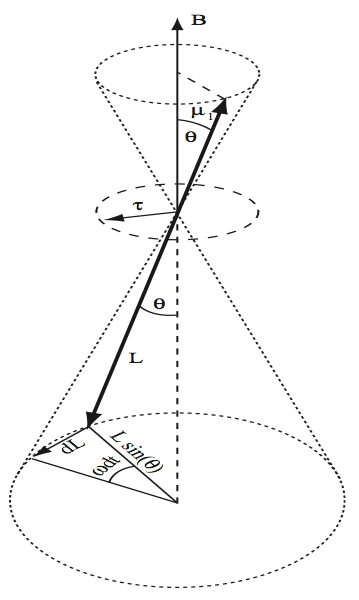
\includegraphics[scale=.5]{../figures/torque}
		\caption{The precession of \dipole about an external \B field.}
	\end{figure}

	Figure 1 provides us with some intuition into how to go about finding the frequency of precession of the dipole moment.  Since we can transform into a rotating frame to describe the motion of $\vec{L}$, we can write
	\begin{gather*}
		\frac{d\vec{L}}{dt} = \vec{\tau} = \vec{\omega} \times \vec{L}\\
		\vec{\mu} \times \vec{B} = \vec{\omega} \times \vec{L}
	\end{gather*}
	and since the angle between \dipole and \B is the same as the angle between $\vec{\omega}$ and $\vec{L}$ by definition of our frame, we can write 
	\begin{gather}
		\omega = \frac{\mu}{L}B\\
		\omega = \gamma B
	\end{gather}
	where $\gamma$ is the gyromagnetic ratio of the object in question.

	\subsection{Quantum System}
	We can express the quantum system and its energy using a simple Hamiltonian.  Since we have an electron precessing in a \B field, we know that $\mathscr{H}$ will be given by
	\begin{gather*}
		\mathscr{H} = \frac{\hat{p}^2}{2m} \nabla^2 + V\\
		\hat{p} = -i\hbar \nabla \rightarrow \hat{p}_{\tiny{e\!f\!f}} = -i\hbar \nabla + \frac{e}{c}A\\
		V = -e\phi\\
	\end{gather*}
	so we can write $\mathscr{H}$ as
	\begin{equation}
		\mathscr{H} = -\frac{\hbar^2}{2m} \nabla^2 -\frac{ie\hbar}{2mc} \big{(}\vec{\nabla}\cdot\vec{A}\big{)} - \frac{ie\hbar}{mc}\big{(}\vec{A}\cdot\vec{\nabla}\big{)} + \frac{e^2}{2mc^2}A^2 - e\phi.
	\end{equation}

	Most often this will be simplified by working in the Coulomb gauge, 
	\begin{equation*}
		\diverg{\vec{A}(\vec{r},t)} = 0
	\end{equation*}
	or the Lorenz gauge,
	\begin{equation*}
		\diverg{\vec{A}} + \frac{1}{c^2}\frac{\partial \phi}{\partial t} = 0.
	\end{equation*}

	In any case, the algebra is trivial yet lengthy and so will be left as an exercise to the reader should they wish.

	\vspace{.25cm}

	Returning to the task at hand, we can define (or derive from the above Hamiltonian, in the first perturbative expansion) the energy of a dipole moment due to an external magnetic field given by
	\begin{equation*}
		E^{(1)} = -\vec{\mu} \cdot \vec{B}
	\end{equation*}
	and so the energy splitting that acts on the free electron will be
	\begin{equation*}
		\Delta E = g_s\mu_B B
	\end{equation*}
	Where $\mu_B$ is the Bohr Magneton, $g_s$ is the dimensionless magnetic moment, and $\Delta E$ is the energy difference between the spin up and spin down states.  Thus if we inject photons with energy $\hbar \omega = \Delta E$ into the system we will be able to force the electron to change spin states.  Since our goal is to measure the gyromagnetic ratio of the electron, we will rewrite the energy shift as follows
	\begin{gather*}
		\hbar \omega = g_s\mu_B B\\
		\omega = \frac{g_s \mu_B}{\hbar} B\\
		\omega = \gamma_e B
	\end{gather*}
	where $\gamma_e$ is the gyromagnetic ratio of the electron. 

	\vspace{.25cm}

	$g_s$ is a dimensionless quantity that is predicted by the Dirac equation to be exactly 2.  However, full quantum electrodynamics introduces small corrections to $g_s$ that can be expressed as
	\begin{equation*}
		g_s = 2\bigg{(}1+\frac{\alpha}{2\pi} + ...\bigg{)}.
	\end{equation*}
	To first order, $g_s = 2$, however.




\section{Apparatus}
	\subsection{Classical System}
	For the classical system the apparatus is shown in figure 2.

	figure here

	We have a billiard ball with an embedded magnet whose moment is aligned along the axis of the small black handle used to spin the ball.  The ball rests on an air mount that simulates a frictionless surface and is centered between two Helmholtz coils that can be controlled to act in parallel or in opposition.  If they act in parallel we can use the relation
	\begin{equation*}
		B = I \times \bigg{(}1.36 \pm 0.003 \hspace{.1cm} \frac{T}{A}\bigg{)}
	\end{equation*}

	In order to actually take data we make use of a strobe light mounted to the Helmholtz coils to track a white dot on the ball's handle as it precesses around the external field.  We also make use of a moveable index to track the ball to measure the period of precession.  While measuring the magnetic moment via the gravitational torque, we use a aluminum rod with a steel end that has a sliding mass mounted to it.  This serves as a means to adjust the torque on the ball due to gravity so that we can measure what \B is required to balance the gravitational force.

	While working through the spin flip portion, we used a saddle that contains fixed permanent magnets to create a \B field perpendicular to the Helmholtz coils.  Spinning this saddle at the correct frequency will create the spin flip phenomenon observed.

	\subsection{Quantum System}
	For the quantum system the apparatus is shown in figure 3.

	figure here

	We use the Deadalon ESR apparatus, consisting of a 60 Hz AC power supply for the large Helmholtz coils, a tunable RF oscillator, and Helmholtz coils connected such that \B at the center will be given by
	\begin{equation*}
		B = I \times \bigg{(}0.48 \hspace{.1cm} \frac{mT}{A}\bigg{)}.
	\end{equation*}
	$I$ is the sum of currents flowing in each coil.  At the center of both the large Helmholtz coils and the RF oscillator is a sample probe containing a small amount of DPPH, a substance containing stable free radicals that allow measurement of the Electron Spin Resonance.  DPPH is typically calibrated so it has a $g_s$ of approximately 2.0036. \cite{DPPH}




\section{Data Analysis}

\section{Error Analysis}

\section{Conclusion}

\begin{thebibliography}{10}
	\bibitem{DPPH}
		McLauchlan, Keith A, et al. \emph{Electron Paramagnetic Resonance: Volume 17 (Specialist Periodic Reports)}, edited by MJ Davies. Royal Society of Chemistry, 2000.
	\bibitem{lab manual}
		University of Chicago Department of Physics. "Introductory Lab: Gamma Cross Sections"\\
		https://wiki.uchicago.edu/display/P211manuals/Introductory+Lab\%3A+Gamma+Cross+Sections. (Accessed Oct 8-16, 2015)

	\bibitem{taylor}
		Taylor, John. \emph{An Introduction to Error Analysis}. Sausalito: University Science Books, 1997.
		
\end{thebibliography}

\end{document}